\documentclass[12pt]{article}
\usepackage[utf8]{inputenc}
\usepackage[utf8]{inputenc}
\usepackage{amsmath}
\usepackage{amsthm}
\usepackage{tabularray}
\usepackage{geometry}
\usepackage{amsfonts}
\usepackage{mathrsfs}
\usepackage{bm}
\usepackage{hyperref}
\usepackage[dvipsnames]{xcolor}
\usepackage{enumitem}
\usepackage{mathtools}
\usepackage{changepage}
\usepackage{lipsum}
\usepackage{tikz}
\usetikzlibrary{matrix}
\usepackage{tikz-cd}
\usepackage[nameinlink]{cleveref}
\geometry{
headheight=15pt,
left=60pt,
right=60pt
}
\setlength{\emergencystretch}{20pt}
\usepackage{fancyhdr}
\pagestyle{fancy}
\fancyhf{}
\lhead{}
\chead{Section 6.A Exercises}
\rhead{\thepage}
\hypersetup{
    colorlinks=true,
    linkcolor=blue,
    urlcolor=blue
}

\theoremstyle{definition}
\newtheorem*{remark}{Remark}

\newtheoremstyle{exercise}
    {}
    {}
    {}
    {}
    {\bfseries}
    {.}
    { }
    {\thmname{#1}\thmnumber{#2}\thmnote{ (#3)}}
\theoremstyle{exercise}
\newtheorem{exercise}{Exercise 6.A.}

\newtheoremstyle{solution}
    {}
    {}
    {}
    {}
    {\itshape\color{magenta}}
    {.}
    { }
    {\thmname{#1}\thmnote{ #3}}
\theoremstyle{solution}
\newtheorem*{solution}{Solution}

\Crefformat{exercise}{#2Exercise 6.A.#1#3}

\newcommand{\re}{\text{Re}\,}
\newcommand{\im}{\text{Im}\,}
\newcommand{\poly}{\mathcal{P}}
\newcommand{\lmap}{\mathcal{L}}
\newcommand{\mat}{\mathcal{M}}
\newcommand{\ts}{\textsuperscript}
\newcommand{\Span}{\text{span}}
\newcommand{\Null}{\text{null\,}}
\newcommand{\Range}{\text{range\,}}
\newcommand{\Rank}{\text{rank\,}}
\newcommand{\quand}{\quad \text{and} \quad}
\newcommand{\ipanon}{\langle \cdot, \cdot \rangle}
\newcommand{\normanon}{\lVert \, \cdot \, \rVert}
\newcommand{\setcomp}[1]{#1^{\mathsf{c}}}
\newcommand{\tpose}[1]{#1^{\text{t}}}
\newcommand{\upd}{\text{d}}
\newcommand{\N}{\mathbf{N}}
\newcommand{\Z}{\mathbf{Z}}
\newcommand{\Q}{\mathbf{Q}}
\newcommand{\R}{\mathbf{R}}
\newcommand{\C}{\mathbf{C}}
\newcommand{\F}{\mathbf{F}}

\DeclarePairedDelimiter\abs{\lvert}{\rvert}
% Swap the definition of \abs* and \norm*, so that \abs
% and \norm resizes the size of the brackets, and the 
% starred version does not.
\makeatletter
\let\oldabs\abs
\def\abs{\@ifstar{\oldabs}{\oldabs*}}

\DeclarePairedDelimiter\norm{\lVert}{\rVert}
\makeatletter
\let\oldnorm\norm
\def\norm{\@ifstar{\oldnorm}{\oldnorm*}}
\makeatother

\DeclarePairedDelimiter\paren{(}{)}
\makeatletter
\let\oldparen\paren
\def\paren{\@ifstar{\oldparen}{\oldparen*}}
\makeatother

\DeclarePairedDelimiter\bkt{[}{]}
\makeatletter
\let\oldbkt\bkt
\def\bkt{\@ifstar{\oldbkt}{\oldbkt*}}
\makeatother

\DeclarePairedDelimiter\set{\{}{\}}
\makeatletter
\let\oldset\set
\def\set{\@ifstar{\oldset}{\oldset*}}
\makeatother

\DeclarePairedDelimiter\ip{\langle}{\rangle}
\makeatletter
\let\oldip\ip
\def\set{\@ifstar{\oldip}{\oldip*}}
\makeatother

\setlist[enumerate,1]{label={(\alph*)}}

\begin{document}

\section{Section 6.A Exercises}

Exercises with solutions from Section 6.A of \hyperlink{ladr}{[LADR]}.

\begin{exercise}
\label{ex:1}
    Show that the function that takes \( ((x_1, x_2), (y_1, y_2)) \in \R^2 \times \R^2 \) to \( \abs{x_1 y_1} + \abs{x_2 y_2} \) is not an inner product on \( \R^2 \).
\end{exercise}

\begin{solution}
    Let \( f \) be the function in question, i.e.\ \( f : \R^2 \times \R^2 \to \R \) is given by
    \[
        f(x, y) = \abs{x_1 y_1} + \abs{x_2 y_2},
    \]
    where \( x = (x_1, x_2) \) and \( y = (y_1, y_2) \). Note that, for \( x = y = (1, 0) \), we have
    \[
        f(-x, y) = 1 \neq -1 = -f(x, y).
    \]
    So \( f \) is not homogeneous in the first argument and hence is not an inner product on \( \R^2 \).
\end{solution}

\begin{exercise}
\label{ex:2}
    Show that the function that takes \( ((x_1, x_2, x_3), (y_1, y_2, y_3)) \in \R^3 \times \R^3 \) to \( x_1 y_1 + x_3 y_3 \) is not an inner product on \( \R^3 \).
\end{exercise}

\begin{solution}
    Let \( f \) be the function in question, i.e.\ \( f : \R^3 \times \R^3 \to \R \) is given by
    \[
        f(x, y) = x_1 y_1 + x_3 y_3,
    \]
    where \( x = (x_1, x_2, x_3) \) and \( y = (y_1, y_2, y_3) \). Let \( x = (0, 1, 0) \). Then \( x \neq 0 \), but
    \[
        f(x, x) = x_1^2 + x_3^2 = 0.
    \]
    So \( f \) is not positive-definite and hence is not an inner product on \( \R^2 \).
\end{solution}

\begin{exercise}
\label{ex:3}
    Suppose \( \F = \R \) and \( V \neq \{ 0 \} \). Replace the positivity condition (which states that \( \ip{v, v} \geq 0 \) for all \( v \in V \)) in the definition of an inner product (6.3) with the condition that \( \ip{v, v} > 0 \) for some \( v \in V \). Show that this change in the definition does not change the set of functions from \( V \times V \) to \( \R \) that are inner products on \( V \).
\end{exercise}

\begin{solution}
    Let us say that a function \( V \times V \) to \( \R \) has property (A) if it satisfies the properties in Definition 6.3, and let us say that a function \( V \times V \) to \( \R \) has property (B) if it satisfies the modified definition in this question. Our aim is to show that a function \( V \times V \) to \( \R \) has property (A) if and only if it has property (B).

    First, suppose that \( \ip{ \cdot, \cdot } : V \times V \to \R \) has property (A). Since \( V \neq \{ 0 \} \), there is some non-zero \( v \in V \). By positivity and definiteness, it must be the case that \( \ip{v, v} > 0 \) and thus \( \ip{ \cdot, \cdot } \) has property (B).

    Now suppose that \( \ip{ \cdot, \cdot } : V \times V \to \R \) has property (B), i.e.\ there exists some \( v \in V \) such that \( \ip{ v, v } > 0 \). We would like to show that \( \ip{ u, u } \geq 0 \) for any \( u \in V \). If \( u \) and \( v \) are linearly dependent, say \( u = \lambda v \) for some scalar \( \lambda \in \R \), then
    \[
        \ip{ u, u } = \lambda^2 \ip{ v, v } \geq 0.
    \]
    Suppose that \( u \) and \( v \) are linearly independent. For \( \lambda \in [0, 1] \), let \( w_{\lambda} = \lambda u + (1 - \lambda) v \). Then
    \[
        \ip{ w_{\lambda}, w_{\lambda} } = \lambda^2 \ip{ u, u } + 2 \lambda (1 - \lambda) \ip{ u, v } + (1 - \lambda)^2 \ip{ v, v }.        
    \]
    Seeking a contradiction, suppose that \( \ip{ u, u } < 0 \). Notice that
    \[
        \ip{ w_0, w_0 } = \ip{ v, v } > 0 \quand \ip{ w_1, w_1 } = \ip{ u, u } < 0.
    \]
    Notice further that \( \ip{ w_{\lambda}, w_{\lambda} } \), as a function of \( \lambda \), is quadratic and hence continuous. We may now appeal to the Intermediate Value Theorem to obtain some \( \lambda' \in (0, 1) \) such that \( \ip{ w_{\lambda'}, w_{\lambda'} } = 0 \). However, since \( u \) and \( v \) are linearly independent, it must be the case that \( w_{\lambda'} \neq 0 \). This contradicts definiteness and we may conclude that \( \ip{ u, u } \geq 0 \) for any \( u \in V \), as desired. Thus \( \ip{ \cdot, \cdot } \) has property (A).
\end{solution}

\begin{exercise}
\label{ex:4}
    Suppose \( V \) is a real inner product space.
    \begin{enumerate}
        \item Show that \( \ip{ u + v, u - v } = \norm{u}^2 - \norm{v}^2 \) for every \( u, v \in V \).

        \item Show that if \( u, v \in V \) have the same norm, then \( u + v \) is orthogonal to \( u - v \).

        \item Use part (b) to show that the diagonals of a rhombus are perpendicular to each other.
    \end{enumerate}
\end{exercise}

\begin{solution}
    \begin{enumerate}
        \item For any \( u, v \in V \) we have
        \[
            \ip{ u + v, u - v } = \ip{ u, u - v } + \ip{ v, u - v } = \ip{ u, u } - \ip{ u, v } + \ip{ v, u } - \ip{ v, v } = \norm{u}^2 - \norm{v}^2.
        \]

        \item This is immediate from part (a).

        \item In plane geometry, a rhombus is a quadrilateral whose four sides have the same length. Letting \( u \) and \( v \) denote the two non-parallel sides, the diagonals are given by \( u + v \) and \( u - v \) (see \Cref{fig:1}). Since \( \norm{u} = \norm{v} \), part (b) implies that \( u + v \) and \( u - v \) are perpendicular to each other.

        \begin{figure}[ht]
            \centering
            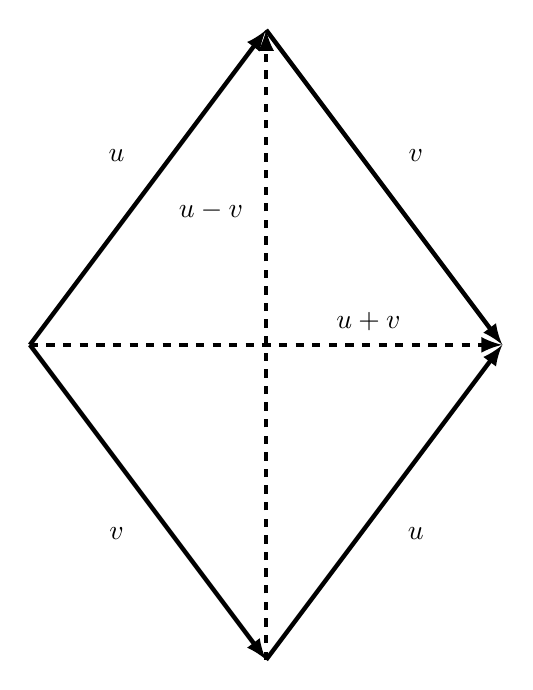
\begin{tikzpicture}
                \draw[ultra thick, -latex] (-3, 0) -- (0, 4);
                \draw[ultra thick, -latex] (-3, 0) -- (0, -4);
                \draw[ultra thick, -latex] (0, 4) -- (3, 0);
                \draw[ultra thick, -latex] (0, -4) -- (3, 0);

                \draw[ultra thick, dashed, -latex] (-3, 0) -- (3, 0);
                \draw[ultra thick, dashed, -latex] (0, -4) -- (0, 4);

                \node at (-1.9, 2.4) {\( u \)};
                \node at (1.9, 2.4) {\( v \)};
                \node at (-1.9, -2.4) {\( v \)};
                \node at (1.9, -2.4) {\( u \)};
                \node at (1.3, 0.3) {\( u + v \)};
                \node at (-0.7, 1.7) {\( u - v \)};
            \end{tikzpicture}
            \caption{Rhombus}
            \label{fig:1}
        \end{figure}
    \end{enumerate}
\end{solution}

\begin{exercise}
\label{ex:5}
    Suppose \( V \) is finite-dimensional (see \href{https://linear.axler.net/LADRErrataThird.html}{errata}) and suppose \( T \in \lmap(V) \) is such that \( \norm{Tv} \leq \norm{v} \) for every \( v \in V \). Prove that \( T - \sqrt{2} I \) is invertible.
\end{exercise}

\begin{solution}
    We will prove the contrapositive statement. Suppose that \( T - \sqrt{2} I \) is not invertible, so that \( T - \sqrt{2} I \) is not injective (3.69), i.e.\ there is some non-zero \( v \in V \) such that \( Tv = \sqrt{2} v \). Then
    \[
        \norm{Tv} = \norm{ \sqrt{2} v } = \sqrt{2} \norm{v} > \norm{v}.
    \]
\end{solution}

\begin{exercise}
\label{ex:6}
    Suppose \( u, v \in V \). Prove that \( \ip{ u, v } = 0 \) if and only if
    \[
        \norm{u} \leq \norm{ u + av }
    \]
    for all \( a \in \F \).
\end{exercise}

\begin{solution}
    Suppose that \( \ip{ u, v } = 0 \) and let \( a \in \F \) be given. Observe that
    \[
        \ip{ u, av } = \overline{a} \ip{ u, v } = 0,
    \]
    so that \( u \) and \( av \) are orthogonal. It follows from the Pythagorean Theorem (6.13) that
    \[
        \norm{u + av}^2 = \norm{u}^2 + \norm{av}^2 \geq \norm{u}^2.
    \]
    Taking square roots gives the desired inequality.

    Now suppose that \( \ip{ u, v } \neq 0 \). By 6.12, it must be the case that \( v \neq 0 \). Thus we can define \( c \) and \( w \) as in 6.14, so that \( \ip{ w, v } = 0 \) and \( u = cv + w \). Since \( w \) and \( v \) are orthogonal, we have by the Pythagorean Theorem (6.13):
    \[
        \norm{u}^2 = \norm{cv + w}^2 = \abs{c}^2 \norm{v}^2 + \norm{w}^2 > \norm{w}^2 = \norm{u - cv}^2;
    \]
    the inequality is strict here since \( c \neq 0 \) and \( v \neq 0 \). Taking square roots gives us \( \norm{u} > \norm{u - cv} \) and so a choice of \( a = -c \) gives us the desired result.
\end{solution}

\begin{exercise}
\label{ex:7}
    Suppose \( u, v \in V \). Prove that \( \norm{au + bv} = \norm{bu + av} \) for all \( a, b \in \R \) if and only if \( \norm{u} = \norm{v} \).
\end{exercise}

\begin{solution}
    For any \( a, b \in \R \), note that \( \norm{au + bv} = \norm{bu + av} \) holds if and only if \( \norm{au + bv}^2 = \norm{bu + av}^2 \). Note further that
    \[
        \norm{au + bv}^2 = a^2 \ip{u, u} + 2ab \ip{u, v} + b^2 \ip{v, v} \quand \norm{bu + av}^2 = b^2 \ip{u, u} + 2ab \ip{u, v} + a^2 \ip{v, v},
    \]
    so that \( \norm{au + bv}^2 = \norm{bu + av}^2 \) holds if and only if
    \[
        (a^2 - b^2)(\ip{u, u} - \ip{v, v}) = 0.
    \]
    Hence it will suffice to show that \( (a^2 - b^2)(\ip{u, u} - \ip{v, v}) = 0 \) for all \( a, b \in \R \) if and only if \( \norm{u} = \norm{v} \). The reverse implication is clear; for the forward implication, simply take \( a = 1 \) and \( b = 0 \).
\end{solution}

\begin{exercise}
\label{ex:8}
    Suppose \( u, v \in V \) and \( \norm{u} = \norm{v} = 1 \) and \( \ip{u, v} = 1 \). Prove that \( u = v \).
\end{exercise}

\begin{solution}
    Observe that
    \[
        \ip{u - v, u - v} = \ip{u, u} - \ip{u, v} - \ip{v, u} + \ip{v, v} = \norm{u}^2 - 2 \text{Re} \ip{u, v} + \norm{v}^2 = 0.
    \]
    Hence by definiteness we must have \( u - v = 0 \).
\end{solution}

\begin{exercise}
\label{ex:9}
    Suppose \( u, v \in V \) and \( \norm{u} \leq 1 \) and \( \norm{v} \leq 1 \). Prove that
    \[
        \sqrt{1 - \norm{u}^2} \sqrt{1 - \norm{v}^2} \leq 1 - \abs{\ip{u, v}}.
    \]
\end{exercise}

\begin{solution}
    Observe that
    \begin{align*}
        0 \leq (\norm{u} - \norm{v})^2 &\iff 0 \leq \norm{u}^2 - 2 \norm{u} \norm{v} + \norm{v}^2 \\[2mm]
        &\iff - \norm{u}^2 - \norm{v}^2 \leq - 2 \norm{u} \norm{v} \\[2mm]
        &\iff 1 - \norm{u}^2 - \norm{v}^2 + \norm{u}^2 \norm{v}^2 \leq 1 - 2 \norm{u} \norm{v} + \norm{u}^2 \norm{v}^2 \\[2mm]
        &\iff \paren{ 1 - \norm{u}^2 } \paren{ 1 - \norm{v}^2 } \leq (1 - \norm{u} \norm{v})^2.
    \end{align*}
    Since \( \norm{u} \leq 1 \) and \( \norm{v} \leq 1 \), the quantities \( 1 - \norm{u}^2, 1 - \norm{v}^2 \), and \( 1 - \norm{u} \norm{v} \) are each non-negative. Thus we may take square roots to obtain the inequality
    \[
        \sqrt{1 - \norm{u}^2} \sqrt{1 - \norm{v}^2} \leq 1 - \norm{u} \norm{v}.
    \]
    It follows from the Cauchy-Schwarz inequality (6.15) that \( 1 - \norm{u} \norm{v} \leq 1 - \abs{\ip{u, v}} \) and thus
    \[
        \sqrt{1 - \norm{u}^2} \sqrt{1 - \norm{v}^2} \leq 1 - \abs{\ip{u, v}}.
    \]
\end{solution}

\begin{exercise}
\label{ex:10}
    Find vectors \( u, v \in \R^2 \) such that \( u \) is a scalar multiple of \( (1, 3), v \) is orthogonal to \( (1, 3) \), and \( (1, 2) = u + v \).
\end{exercise}

\begin{solution}
    Let \( x = (1, 2), y = (1, 3) \) and set
    \[
        c = \frac{\ip{x, y}}{\norm{y}^2} = \frac{7}{10}, \quad u = cy, \quand v = x - cy.
    \]
    Then \( u \) is a scalar multiple of \( y \) and, as 6.14 shows, we have \( \ip{v, y} = 0 \) and \( x = u + v \).
\end{solution}

\begin{exercise}
\label{ex:11}
    Prove that
    \[
        16 \leq (a + b + c + d) \paren{ \frac{1}{a} + \frac{1}{b} + \frac{1}{c} + \frac{1}{d} }
    \]
    for all positive numbers \( a, b, c, d \).
\end{exercise}

\begin{solution}
    Let
    \[
        u = \paren{ \sqrt{a}, \sqrt{b}, \sqrt{c}, \sqrt{d} } \quand v = \paren{ \frac{1}{\sqrt{a}}, \frac{1}{\sqrt{b}}, \frac{1}{\sqrt{c}}, \frac{1}{\sqrt{d}} }.
    \]
    Then
    \[
        \ip{u, v} = 4, \quad \norm{u} = \sqrt{a + b + c + d}, \quand \norm{v} = \sqrt{\frac{1}{a} + \frac{1}{b} + \frac{1}{c} + \frac{1}{d}}.
    \]
    Squaring both sides of the Cauchy-Schwarz inequality (6.15) gives the desired inequality.
\end{solution}

\begin{exercise}
\label{ex:12}
    Prove that
    \[
        (x_1 + \cdots + x_n)^2 \leq n (x_1^2 + \cdots + x_n^2)
    \]
    for all positive integers \( n \) and all real numbers \( x_1, \ldots, x_n \).
\end{exercise}

\begin{solution}
    Let \( n \) be a positive integer, \( x_1, \ldots, x_n \) be real numbers, and set
    \[
        u = (1, \ldots, 1) \in \R^n \quand v = (x_1, \ldots, x_n) \in \R^n.
    \]
    Then
    \[
        \ip{u, v} = x_1 + \cdots + x_n, \quad \norm{u} = \sqrt{n}, \quand \norm{v} = \sqrt{x_1^2 + \cdots + x_n^2}.
    \]
    Squaring both sides of the Cauchy-Schwarz inequality (6.15) gives the desired inequality.
\end{solution}

\begin{exercise}
\label{ex:13}
    Suppose \( u, v \) are nonzero vectors in \( \R^2 \). Prove that
    \[
        \ip{u, v} = \norm{u} \norm{v} \cos \theta,
    \]
    where \( \theta \) is the angle between \( u \) and \( v \) (thinking of \( u \) and \( v \) as arrows with initial point at the origin).

    \vspace{1mm}

    \noindent \textit{Hint:} Draw the triangle formed by \( u, v, \) and \( u - v \); then use the law of cosines.
\end{exercise}

\begin{solution}
    \begin{figure}[ht]
        \centering
        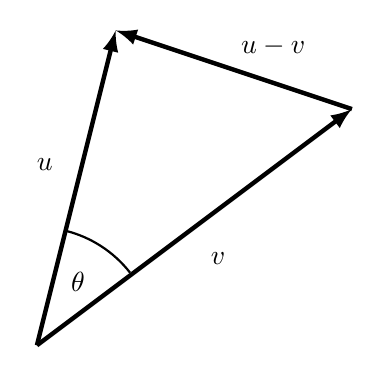
\begin{tikzpicture}
            \draw[ultra thick, -latex] (0, 0) -- (1, 4);
            \draw[ultra thick, -latex] (0, 0) -- (4, 3);
            \draw[ultra thick, -latex] (4, 3) -- (1, 4);
            \draw[thick] (38:1.5) arc (38:76:1.5);


            \node at (0.1, 2.3) {\( u \)};
            \node at (2.3, 1.1) {\( v \)};
            \node at (3, 3.8) {\( u - v \)};
            \node at (0.52, 0.8) {\( \theta \)};
        \end{tikzpicture}
        \caption{Triangle}
        \label{fig:2}
    \end{figure}

    Following the hint, consider the triangle in \Cref{fig:2}. The law of cosines states that
    \[
        \norm{u - v}^2 = \norm{u}^2 + \norm{v}^2 - 2 \norm{u} \norm{v} \cos \theta.
    \]
    Equivalently,
    \[
        \ip{u - v, u - v} = \ip{u, u} + \ip{v, v} - 2 \norm{u} \norm{v} \cos \theta. 
    \]
    After expanding \( \ip{u - v, u - v} \), we find the desired equality.
\end{solution}

\begin{exercise}
\label{ex:14}
    The angle between two vectors (thought of as arrows with initial point at the origin) in \( \R^2 \) or \( \R^3 \) can be defined geometrically. However, geometry is not as clear in \( \R^n \) for \( n > 3 \). Thus the angle between two nonzero vectors \( x, y \in \R^n \) is defined to be
    \[
        \arccos \frac{\ip{x, y}}{\norm{x} \norm{y}},
    \]
    where the motivation for this definition comes from the previous exercise. Explain why the Cauchy-Schwarz Inequality is needed to show that this definition makes sense.
\end{exercise}

\begin{solution}
    The \( \arccos \) function is defined on the interval \( [-1, 1] \); for the definition in question to make sense, we must have
    \[
        \frac{\ip{x, y}}{\norm{x} \norm{y}} \in [-1, 1]
    \]
    for any non-zero \( x, y \in \R^n \). The Cauchy-Schwarz inequality ensures this.
\end{solution}

\begin{exercise}
\label{ex:15}
    Prove that
    \[
        \paren{ \sum_{j=1}^n a_j b_j }^2 \leq \paren{ \sum_{j=1}^n j a_j^2 } \paren{ \sum_{j=1}^n \frac{b_j^2}{j} }  
    \]
    for all real numbers \( a_1, \ldots, a_n \) and \( b_1, \ldots, b_n \).
\end{exercise}

\begin{solution}
    Let \( n \) be a positive integer and let \( a_1, \ldots, a_n, b_1, \ldots, b_n \) be real numbers. Define
    \[
        u = \paren{ a_1, \sqrt{2} a_2, \sqrt{3} a_3, \ldots, \sqrt{n} a_n } \quand v = \paren{ b_1, \frac{b_2}{\sqrt{2}}, \frac{b_3}{\sqrt{3}}, \ldots, \frac{b_n}{\sqrt{n}} }.
    \]
    Then
    \[
        \ip{u, v} = \sum_{j=1}^n a_j b_j, \quad \norm{u} = \paren{ \sum_{j=1}^n j a_j^2 }^{1/2}, \quand \norm{v} = \paren{ \sum_{j=1}^n \frac{b_j^2}{j} }^{1/2}.
    \]
    Squaring both sides of the Cauchy-Schwarz inequality (6.15) gives the desired inequality.
\end{solution}

\begin{exercise}
\label{ex:16}
    Suppose \( u, v \in V \) are such that
    \[
        \norm{u} = 3, \quad \norm{u + v} = 4, \quad \norm{u - v} = 6.
    \]
    What number does \( \norm{v} \) equal?
\end{exercise}

\begin{solution}
    Rearranging the parallelogram equality (6.22) for \( \norm{v} \) gives
    \[
        \norm{v} = \paren{ \frac{\norm{u + v}^2 + \norm{u - v}^2}{2} - \norm{u}^2 }^{1/2}.
    \]
    Substituting the given values, we find \( \norm{v} = \sqrt{17} \).
\end{solution}

\begin{exercise}
\label{ex:17}
    Prove or disprove: there is an inner product on \( \R^2 \) such that the associated norm is given by
    \[
        \norm{(x, y)} = \max \{ \abs{x}, \abs{y} \}
    \]
    (see \href{https://linear.axler.net/LADRErrataThird.html}{errata}) for all \( (x, y) \in \R^2 \).
\end{exercise}

\begin{solution}
    There is no such inner product. Let \( f : \R^2 \to \R \) be given by \( f(x, y) = \max \{ \abs{x}, \abs{y} \} \). If \( f \) was indeed a norm arising from an inner product, then \( f \) would satisfy the parallelogram equality (6.22). However, let \( u = (1, 0) \) and \( v = (1, 1) \). Then
    \[
        [f(u + v)]^2 + [f(u - v)]^2 = 5 \neq 4 = 2 \paren{ [f(u)]^2 + [f(v)]^2 }.
    \]
\end{solution}

\begin{exercise}
\label{ex:18}
    Suppose \( p > 0 \). Prove that there is an inner product on \( \R^2 \) such that the associated norm is given by
    \[
        \norm{(x, y)} = \paren{\abs{x}^p + \abs{y}^p}^{1/p}
    \]
    (see \href{https://linear.axler.net/LADRErrataThird.html}{errata}) for all \( (x, y) \in \R^2 \) if and only if \( p = 2 \).
\end{exercise}

\begin{solution}
    Let \( f : \R^2 \to \R \) be given by \( f(x, y) = \paren{\abs{x}^p + \abs{y}^p}^{1/p} \). If \( f \) was indeed a norm arising from an inner product, then \( f \) would satisfy the parallelogram equality (6.22). Let \( u = (1, 0) \) and \( v = (0, 1) \). Then
    \[
        [f(u + v)]^2 + [f(u - v)]^2 = 2^{1 + 2/p} \quand 2 \paren{ [f(u)]^2 + [f(v)]^2 } = 4.
    \]
    These are equal if and only if \( 2^{2/p} = 2 \), which is the case if and only if \( p = 2 \). Thus the only possible value for \( p \) is 2, which indeed gives the norm arising from the Euclidean inner product on \( \R^2 \) (see Example 6.9 (a)).
\end{solution}

\begin{exercise}
\label{ex:19}
    Suppose \( V \) is a real inner product space. Prove that
    \[
        \ip{u, v} = \frac{\norm{u + v}^2 - \norm{u - v}^2}{4}
    \]
    for all \( u, v \in V \).
\end{exercise}

\begin{solution}
    Let \( u, v \in V \) be given. Then
    \begin{align*}
        \norm{u + v}^2 - \norm{u - v}^2 &= \ip{u + v, u + v} - \ip{u - v, u - v} \\[2mm]
        &= \ip{u, u} + 2 \ip{u, v} + \ip{v, v} - \ip{u, u} + 2 \ip{u, v} - \ip{v, v} \\[2mm]
        &= 4 \ip{u, v}.
    \end{align*}
\end{solution}

\begin{exercise}
\label{ex:20}
    Suppose \( V \) is a complex inner product space. Prove that
    \[
        \ip{u, v} = \frac{\norm{u + v}^2 - \norm{u - v}^2 + \norm{u + iv}^2 i - \norm{u - iv}^2 i}{4}
    \]
    for all \( u, v \in V \).
\end{exercise}

\begin{solution}
    Let \( u, v \in V \) be given. Then
    \begin{align*}
        \norm{u + v}^2 - \norm{u - v}^2 &= \ip{u + v, u + v} - \ip{u - v, u - v} \\[2mm]
        &= \ip{u, u} + \ip{u, v} + \overline{\ip{u, v}} + \ip{v, v} \\[2mm]
        &- \ip{u, u} + \ip{u, v} + \overline{\ip{u, v}} - \ip{v, v} \\[2mm]
        &= 2 \paren{ \ip{u, v} + \overline{\ip{u, v}} } \\[2mm]
        &= 4 \text{Re} \ip{u, v}.
    \end{align*}
    Furthermore,
    \begin{align*}
        i \norm{u + iv}^2 - i \norm{u - iv}^2 &= i \ip{u + iv, u + iv} - i \ip{u - iv, u - iv} \\[2mm]
        &= i \ip{u, u} - i^2 \ip{u, v} + i^2 \overline{\ip{u, v}} + i \ip{v, v} \\[2mm]
        &- i \ip{u, u} - i^2 \ip{u, v} + i^2 \overline{\ip{u, v}} - i \ip{v, v} \\[2mm]
        &= 2 \paren{ \ip{u, v} - \overline{\ip{u, v}} } \\[2mm]
        &= 4 \text{Im} \ip{u, v}.
    \end{align*}
    It follows that
    \[
        \norm{u + v}^2 - \norm{u - v}^2 + i \norm{u + iv}^2 - i \norm{u - iv}^2 = 4 \ip{u, v}.
    \]
\end{solution}

\begin{exercise}
\label{ex:21}
    A norm on a vector space \( U \) is a function \( \norm{\,\,} : U \to [0, \infty) \) such that \( \norm{u} = 0 \) if and only if \( u = 0 \), \( \norm{\alpha u} = \abs{a} \norm{u} \) for all \( \alpha \in \F \) and all \( u \in U \), and \( \norm{u + v} \leq \norm{u} + \norm{v} \) for all \( u, v \in U \). Prove that a norm satisfying the parallelogram equality comes from an inner product (in other words, show that if \( \norm{\,\,} \) is a norm on \( U \) satisfying the parallelogram equality, then there is an inner product \( \ip{\, , \,} \) on \( U \) such that \( \norm{u} = \ip{u, u}^{1/2} \) for all \( u \in U \)).
\end{exercise}

\begin{solution}
    Let us first consider the case where \( U \) is a real vector space. Define \( \ipanon : U \times U \to \R \) by
    \[
        \ip{u, v} = \frac{\norm{u + v}^2 - \norm{u - v}^2}{4}.
    \]
    For any \( u \in U \), we have
    \[
        \ip{u, u} = \frac{\norm{2u}^2}{4} = \norm{u}^2.
    \]
    From this expression, we can see that the norm is given by \( \norm{u} = \ip{u, u}^{1/2} \). It remains to show that \( \ipanon \) satisfies the properties of an inner product given in 6.3.
    \begin{description}
        \item[Positive-definiteness.] Combining the identity \( \ip{u, u} = \norm{u}^2 \) with the properties of a norm shows that \( \ipanon \) is positive-definite.

        \item[Symmetry.] Simply observe that \( \norm{v - u} = \norm{u - v} \).

        \item[Additivity in the first slot.] Let \( u, v, w \in U \) be given. Since \( \normanon \) satisfies the parallelogram equality, we have
        \begin{align*}
            \norm{v + 2w}^2 + \norm{v}^2 &= 2 \norm{v + w}^2 + 2 \norm{w}^2, \\[2mm]
            \norm{v - 2w}^2 + \norm{v}^2 &= 2 \norm{v - w}^2 + 2 \norm{w}^2.
        \end{align*}
        Subtracting the latter of these equations from the former gives us
        \[
            \norm{v + 2w}^2 - \norm{v - 2w}^2 = 2 \norm{v + w}^2 - 2 \norm{v - w}^2. \tag{1}
        \]
        Now we use the parallelogram equality two more times:
        \begin{align*}
            2 \norm{u + v + w}^2 + 2 \norm{u - w}^2 &= \norm{v + 2u}^2 + \norm{v + 2w}^2 \\[2mm]
            2 \norm{u + v - w}^2 + 2 \norm{u + w}^2 &= \norm{v + 2u}^2 + \norm{v - 2w}^2.
        \end{align*}
        Subtracting the latter of these equations from the former gives us
        \[
            2(\norm{u + v + w}^2 + \norm{u - w}^2) - 2(\norm{u + v - w}^2 + \norm{u + w}^2) = \norm{v + 2w}^2 - \norm{v - 2w}^2.
        \]
        Combining this with equation (1), we see that
        \[
            2(\norm{u + v + w}^2 + \norm{u - w}^2) - 2(\norm{u + v - w}^2 + \norm{u + w}^2) = 2 \norm{v + w}^2 - 2 \norm{v - w}^2.
        \]
        Equivalently,
        \[
            \frac{\norm{u + v + w}^2 - \norm{u + v - w}^2}{4} = \frac{\norm{u + w}^2 - \norm{u - w}^2 + \norm{v + w}^2 - \norm{v - w}^2}{4},
        \]
        which is exactly the statement \( \ip{u + v, w} = \ip{u, w} + \ip{v, w} \).

        \item[Homogeneity in the first slot.] Suppose \( u, v \in U \). We will first prove by induction that \( \ip{nu, v} = n \ip{u, v} \) for all positive integers \( n \). The base case \( n = 1 \) is clear, so suppose that the result holds for some positive integer \( n \). Then
        \[
            \ip{(n + 1)u, v} = \ip{nu + u, v} = \ip{nu, v} + \ip{u, v} = n \ip{u, v} + \ip{u, v} = (n + 1) \ip{u, v},
        \]
        where we have used additivity in the first slot and the induction hypothesis. This completes the induction step and thus we have homogeneity in the first slot for all positive integers. It is clear that \( \ip{0, v} = 0 \) and so we may extend this result to all non-negative integers. If \( n \) is a positive integer, then observe that
        \[
            \ip{-nu, v} + n \ip{u, v} = \ip{-nu, v} + \ip{nu, v} = \ip{0, v} = 0,
        \]
        where we have used additivity in the first slot and homogeneity in the first slot for positive integers. It follows that \( \ip{-nu, v} = -n \ip{u, v} \) and thus we have homogeneity in the first slot for all integers.
    
        To extend homogeneity in the first slot to rational numbers, let \( n \) be a positive integer. Then by additivity in the first slot, we have
        \[
            n \ip{n^{-1} u, v} = \sum_{j=1}^n \ip{n^{-1} u, v} = \ip*{\textstyle{\sum_{j=1}^n n^{-1} u, v}} = \ip{u, v},
        \]
        which implies that \( \ip{n^{-1} u, v} = n^{-1} \ip{u, v} \). Combining this with homogeneity in the first slot for integers allows us to extend the result to rational numbers.
    
        Finally, to obtain homogeneity in the first slot for all real numbers, let \( \lambda \in \R \) be given. By the density of \( \Q \) in \( \R \), there exists a sequence \( (r_n) \) of rational numbers satisfying \( \lim_{n \to \infty} r_n = \lambda \). The \href{https://en.wikipedia.org/wiki/Triangle_inequality#Reverse_triangle_inequality}{reverse triangle inequality} is readily deduced from the triangle inequality and allows one to establish the continuity of the function \( u \mapsto \norm{u} \). Given this, and standard results on compositions and linear combinations of continuous functions, we have
        \begin{align*}
            \lambda \ip{u, v} &= \lim_{n \to \infty} r_n \ip{u, v} \\[2mm]
            &= \lim_{n \to \infty} \ip{r_n u, v} \\[2mm]
            &= \lim_{n \to \infty} \frac{\norm{r_n u + v}^2 - \norm{r_n u - v}^2}{4} \\[2mm]
            &= \frac{\norm{\lambda u + v}^2 - \norm{\lambda u - v}^2}{4} \\[2mm]
            &= \ip{\lambda u, v}.
        \end{align*}
    \end{description}
    Now let us consider the case where \( U \) is a complex vector space. Define \( B : U \times U \to \R \) by
    \[
        B(u, v) = \frac{\norm{u + v}^2 - \norm{u - v}^2}{4}
    \]
    and define \( \ipanon : U \times U \to \C \) by
    \[
        \ip{u, v} = B(u, v) + i B(u, iv) = \frac{\norm{u + v}^2 - \norm{u - v}^2}{4} + i \frac{\norm{u + iv}^2 - \norm{u - iv}^2}{4}.
    \]
    Observe that for any \( u \in U \) we have \( B(u, u) = \norm{u}^2 \) and
    \[
        B(u, iu) = \frac{\norm{u + iu}^2 - \norm{u - iu}^2}{4} = \frac{\abs{1 + i}^2 \norm{u}^2 - \abs{1 - i}^2 \norm{u}^2}{4} = 0.
    \]
    Thus \( \ip{u, u} = \norm{u}^2 \). From this expression, we can see that the norm is given by \( \norm{u} = \ip{u, u}^{1/2} \). It remains to show that \( \ipanon \) satisfies the properties of an inner product given in 6.3.
    
    \begin{description}
        \item[Positive-definiteness.] Combining the identity \( \ip{u, u} = \norm{u}^2 \) with the properties of a norm shows that \( \ipanon \) is positive-definite.

        \item[Conjugate symmetry.] For any \( u, v \in U \), note that
        \[
            \overline{\ip{v, u}} = \overline{B(v, u) + i B(v, iu)} = B(u, v) - i B(v, iu),
        \]
        where we have used that \( B \) is real-valued and symmetric. Given the expression above, to verify conjugate symmetry of \( \ipanon \) it will suffice to show that \( B(u, iv) = -B(v, iu) \). Indeed,
        \begin{multline*}
            -4 B(v, iu) = \norm{v - iu}^2 - \norm{v + iu}^2 = \norm{-i(u + iv)}^2 - \norm{i(u - iv)}^2 \\[2mm]
            = \abs{-i}^2 \norm{u + iv}^2 - \abs{i}^2 \norm{u - iv}^2 = \norm{u + iv}^2 - \norm{u - iv}^2 = 4 B(u, iv).
        \end{multline*}

        \item[Additivity in the first slot.] Let \( u, v, w \in U \) be given. Observe that the proof of additivity in the first slot we gave for the case where \( U \) is a real vector space equally shows that \( B \) is additive in the first slot. It follows that
        \begin{multline*}
            \ip{u + v, w} = B(u + v, w) + i B(u + v, iw) \\
            = B(u, w) + i B(u, iw) + B(v, w) + i B(v, iw) = \ip{u, w} + \ip{v, w}.
        \end{multline*}

        \item[Homogeneity in the first slot.] Let \( u, v \in U \) be given. Observe that the proof of homogeneity in the first slot we gave for the case where \( U \) is a real vector space equally shows that \( B \) is homogeneous in the first slot with respect to real numbers. It follows that for any \( \lambda \in \R \) we have \( \ip{\lambda u, v} = \lambda \ip{u, v} \). Now observe that
        \begin{align*}
            \ip{iu, v} &= \frac{\norm{iu + v}^2 - \norm{iu - v}^2}{4} + i \frac{\norm{iu + iv}^2 - \norm{iu - iv}^2}{4} \\[2mm]
            &= \frac{\norm{i(u - iv)}^2 - \norm{i(u + iv)}^2}{4} + i \frac{\norm{i(u + v)}^2 - \norm{i(u - v)}^2}{4} \\[2mm]
            &= \frac{\norm{u - iv}^2 - \norm{u + iv}^2}{4} + i \frac{\norm{u + v}^2 - \norm{u - v}^2}{4} \\[2mm]
            &= i \paren{ \frac{\norm{u + v}^2 - \norm{u - v}^2}{4} + i \frac{\norm{u + iv}^2 - \norm{u - iv}^2}{4} } \\[2mm]
            &= i \ip{u, v}.
        \end{align*}
        Let \( x + iy \in \C \) be given. Then
        \[
            \ip{(x + iy)u, v} = \ip{xu + iyu, v} = \ip{xu, v} + \ip{iyu, v} = x \ip{u, v} + iy \ip{u, v} = (x + iy) \ip{u, v}.
        \]
    \end{description}
\end{solution}

\begin{exercise}
\label{ex:22}
    Show that the square of an average is less than or equal to the average of the squares. More precisely, show that if \( a_1, \ldots, a_n \in \R \), then the square of the average of \( a_1, \ldots, a_n \) is less than or equal to the average of \( a_1^2, \ldots, a_n^2 \).
\end{exercise}

\begin{solution}
    For a positive integer \( n \) and real numbers \( a_1, \ldots, a_n \), let
    \[
        u = (a_1, \ldots, a_n) \in \R^n \quand v = \paren{ \frac{1}{n}, \ldots, \frac{1}{n} } \in \R^n.
    \]
    Then
    \[
        \ip{u, v}^2 = \paren{\frac{a_1 + \cdots + a_n}{n}}^2, \quad \norm{u}^2 = a_1^2 + \cdots + a_n^2, \quand \norm{v}^2 = \frac{1}{n}.
    \]
    Squaring both sides of the Cauchy-Schwarz inequality (6.15) gives the desired inequality.
\end{solution}

\begin{exercise}
\label{ex:23}
    Suppose \( V_1, \ldots, V_m \) are inner product spaces. Show that the equation
    \[
        \ip{(u_1, \ldots, u_m), (v_1, \ldots, v_m)} = \ip{u_1, v_1} + \cdots + \ip{u_m, v_m}
    \]
    defines an inner product on \( V_1 \times \cdots \times V_m \).

    \noindent [\textit{In the expression above on the right, \( \ip{u_1, v_1} \) denotes the inner product on \( V_1, \ldots, \ip{u_m, v_m} \) denotes the inner product on \( V_m \). Each of the spaces \( V_1, \ldots, V_m \) may have a different inner product, even though the same notation is used here.}]
\end{exercise}

\begin{solution}
    For convenience, let \( \mathbf{V} = V_1 \times \cdots \times V_m \). It is clear that the equation in question gives a well-defined function \( \mathbf{V} \times \mathbf{V} \to \F \). It remains to show that the properties of an inner product are satisfied.
    \begin{description}
        \item[Positivity.] Let \( (v_1, \ldots, v_m) \in \mathbf{V} \) be given. Then
        \[
            \ip{(v_1, \ldots, v_m), (v_1, \ldots, v_m)} = \ip{v_1, v_1} + \cdots + \ip{v_m, v_m}.
        \]
        Since each \( \ip{v_j, v_j} \) is non-negative, it follows that \( \ip{(v_1, \ldots, v_m), (v_1, \ldots, v_m)} \) is also non-negative.

        \item[Definiteness.] Note that \( (v_1, \ldots, v_m) = 0 \) if and only if each \( v_j = 0 \). By the definiteness of the inner product on each \( V_j \), this is the case if and only if each \( \ip{v_j, v_j} = 0 \). From the non-negativity of the expression
        \[
            \ip{(v_1, \ldots, v_m), (v_1, \ldots, v_m)} = \ip{v_1, v_1} + \cdots + \ip{v_m, v_m},
        \]
        we see that each \( \ip{v_j, v_j} = 0 \) if and only if \( \ip{(v_1, \ldots, v_m), (v_1, \ldots, v_m)} = 0 \).

        \item[Additivity in first slot.] Let \( (u_1, \ldots, u_m), (v_1, \ldots, v_m), (w_1, \ldots, w_m) \in \mathbf{V} \) be given. Then
        \begin{align*}
            & \quad\,\, \ip{(u_1, \ldots, u_m) + (v_1, \ldots, v_m), (w_1, \ldots, w_m)} \\[2mm]
            &= \ip{(u_1 + v_1, \ldots, u_m + v_m), (w_1, \ldots, w_m)} \\[2mm]
            &= \ip{u_1 + v_1, w_1} + \cdots + \ip{u_m + v_m, w_m} \\[2mm]
            &= \ip{u_1, w_1} + \ip{v_1, w_1} + \cdots + \ip{u_m, w_m} + \ip{v_m, w_m} \\[2mm]
            &= \ip{u_1, w_1} + \cdots + \ip{u_m, w_m} + \ip{v_1, w_1} + \cdots + \ip{v_m, w_m} \\[2mm]
            &= \ip{(u_1, \ldots, u_m), (w_1, \ldots, w_m)} + \ip{(v_1, \ldots, v_m), (w_1, \ldots, w_m)},
        \end{align*}
        where we have used the additivity in the first slot of the inner product on each \( V_j \).

        \item[Homogeneity in first slot.] Let \( \lambda \in \F \) and \( (u_1, \ldots, u_m), (v_1, \ldots, v_m) \in \mathbf{V} \) be given. Then
        \begin{align*}
            \ip{\lambda (u_1, \ldots, u_m), (v_1, \ldots, v_m)} &= \ip{(\lambda u_1, \ldots, \lambda u_m), (v_1, \ldots, v_m)} \\[2mm]
            &= \ip{\lambda u_1, v_1} + \cdots + \ip{\lambda u_m, v_m} \\[2mm]
            &= \lambda \ip{u_1, v_1} + \cdots + \lambda \ip{u_m, v_m} \\[2mm]
            &= \lambda (\ip{u_1, v_1} + \cdots + \ip{u_m, v_m}) \\[2mm]
            &= \lambda \ip{(u_1, \ldots, u_m), (v_1, \ldots, v_m)},
        \end{align*}
        where we have used the homogeneity in the first slot of the inner product on each \( V_j \).

        \item[Conjugate symmetry.] Let \( (u_1, \ldots, u_m), (v_1, \ldots, v_m) \in \mathbf{V} \) be given. Then
        \begin{align*}
            \overline{\ip{(v_1, \ldots, v_m), (u_1, \ldots, u_m)}} &= \overline{\ip{v_1, u_1} + \cdots + \ip{v_m, u_m}} \\[2mm]
            &= \overline{\ip{v_1, u_1}} + \cdots + \overline{\ip{v_m, u_m}} \\[2mm]
            &= \ip{u_1, v_1} + \cdots + \ip{u_m, v_m} \\[2mm]
            &= \ip{(u_1, \ldots, u_m), (v_1, \ldots, v_m)},
        \end{align*}
        where we have used the conjugate symmetry of the inner product on each \( V_j \).
    \end{description}
\end{solution}

\begin{exercise}
\label{ex:24}
    Suppose \( S \in \lmap(V) \) is an injective operator on \( V \). Define \( \ipanon_1 \) by
    \[
        \ip{u, v}_1 = \ip{Su, Sv}
    \]
    for \( u, v \in V \). Show that \( \ipanon_1 \) is an inner product on \( V \).
\end{exercise}

\begin{solution}
    It is clear that the definition in question gives a well-defined function \( V \times V \to \F \). It remains to show that the properties of an inner product are satisfied.
    \begin{description}
        \item[Positivity.] We have \( \ip{v, v}_1 = \ip{Sv, Sv} \geq 0 \) by the positivity of \( \ipanon \).

        \item[Definiteness.] Note that \( \ip{v, v}_1 = \ip{Sv, Sv} = 0 \) if and only if \( Sv = 0 \) by the definiteness of \( \ipanon \), and \( Sv = 0 \) if and only if \( v = 0 \) by the injectivity of \( S \).

        \item[Additivity in the first slot.] Let \( u, v, w \in V \) be given. Then
        \[
            \ip{u + v, w}_1 = \ip{S(u + v), Sw} = \ip{Su + Sv, Sw} = \ip{Su, Sw} + \ip{Sv, Sw} = \ip{u, w}_1 + \ip{v, w}_1,
        \]
        where we have used the linearity of \( S \) and the additivity in the first slot of \( \ipanon \).

        \item[Homogeneity in the first slot.] Let \( \lambda \in \F \) and \( u, v \in V \) be given. Then
        \[
            \ip{\lambda u, v}_1 = \ip{S(\lambda u), Sv} = \ip{\lambda Su, Sv} = \lambda \ip{Su, Sv} = \lambda \ip{u, v}_1,
        \]
        where we have used the linearity of \( S \) and the homogeneity in the first slot of \( \ipanon \).

        \item[Conjugate symmetry.] Let \( u, v \in V \) be given. Then
        \[
            \overline{\ip{v, u}_1} = \overline{\ip{Sv, Su}} = \ip{Su, Sv} = \ip{u, v}_1,
        \]
        where we have used the conjugate symmetry of \( \ipanon \).
    \end{description}
\end{solution}

\begin{exercise}
\label{ex:25}
    Suppose \( S \in \lmap(V) \) is not injective. Define \( \ipanon_1 \) as in the exercise above. Explain why \( \ipanon_1 \) is not an inner product on \( V \).
\end{exercise}

\begin{solution}
    Since \( S \) is not injective, there exists some non-zero \( v \in V \) such that \( Sv = 0 \). Then
    \[
        \ip{v, v}_1 = \ip{Sv, Sv} = \ip{0, 0} = 0,  
    \]
    so that \( \ipanon_1 \) is not definite.
\end{solution}

\begin{exercise}
\label{ex:26}
    Suppose \( f, g \) are differentiable functions from \( \R \) to \( \R^n \).
    \begin{enumerate}
        \item Show that
        \[
            \ip{f(t), g(t)}' = \ip{f'(t), g(t)} + \ip{f(t), g'(t)}.
        \]

        \item Suppose \( c > 0 \) and \( \norm{f(t)} = c \) for every \( t \in \R \). Show that \( \ip{f'(t), f(t)} = 0 \) for every \( t \in \R \).

        \item Interpret the result in part (b) geometrically in terms of the tangent vector to a curve lying on a sphere in \( \R^n \) centered at the origin.
    \end{enumerate}

    \noindent [\textit{For the exercise above, a function \( f : \R \to \R^n \) is called differentiable if there exist differentiable functions \( f_1, \ldots, f_n \) from \( \R \) to \( \R \) such that \( f(t) = (f_1(t), \ldots, f_n(t)) \) for each \( t \in \R \). Furthermore, for each \( t \in \R \), the derivative \( f'(t) \in \R^n \) is defined by \( f'(t) = (f_1'(t), \ldots, f_n'(t)) \).}]
\end{exercise}

\begin{solution}
    \begin{enumerate}
        \item Suppose that \( f(t) = (f_1(t), \ldots, f_n(t)) \) and \( g(t) = (g_1(t), \ldots, g_n(t)) \) for some differentiable functions \( f_1, \ldots, f_n, g_1, \ldots, g_n : \R \to \R \). Then we have by the usual rules of differentiation:
        \begin{align*}
            \ip{f(t), g(t)}' &= (f_1(t) g_1(t) + \cdots + f_n(t) g_n(t))' \\[2mm]
            &= f_1'(t) g_1(t) + f_1(t) g_1'(t) + \cdots + f_n'(t) g_n(t) + f_n(t) g_n'(t) \\[2mm]
            &= f_1'(t) g_1(t) + \cdots + f_n'(t) g_n(t) + f_1(t) g_1'(t) + \cdots + f_n(t) g_n'(t) \\[2mm]
            &= \ip{f'(t), g(t)} + \ip{f(t), g'(t)}.
        \end{align*}

        \item By part (a), we have
        \[
            0 = \paren{ c^2 }' = \paren{ \norm{f(t)}^2 }' = \ip{f(t), f(t)}' = 2 \ip{f'(t), f(t)}.
        \]
        Thus \( \ip{f'(t), f(t)} = 0 \).

        \item Suppose \( c > 0 \). A differentiable function \( f : \R \to \R^n \) satisfying \( \norm{f(t)} = c \) for every \( t \in \R \) traces out a curve which lies on an \( (n - 1) \)-sphere of radius \( c \) centered at the origin in \( \R^n \). The tangent vector to this curve is given by \( f' \); the result of part (b) states that this tangent vector is always orthogonal to the curve \( f \).
    \end{enumerate}
\end{solution}

\begin{exercise}
\label{ex:27}
    Suppose \( u, v, w \in V \). Prove that
    \[
        \norm{w - \tfrac{1}{2}(u + v)}^2 = \frac{\norm{w - u}^2 + \norm{w - v}^2}{2} - \frac{\norm{u - v}^2}{4}.
    \]
\end{exercise}

\begin{solution}
    It will suffice to prove that
    \[
        4 \norm{w - \tfrac{1}{2}(u + v)}^2 = 2 \paren{ \norm{w - u}^2 + \norm{w - v}^2 } - \norm{u - v}^2,
    \]
    which is equivalent to
    \[
        \norm{2w - u - v}^2 + \norm{u - v}^2 = 2 \paren{ \norm{w - u}^2 + \norm{w - v}^2 }.
    \]
    This follows immediately from the parallelogram equality.
\end{solution}

\begin{exercise}
\label{ex:28}
    Suppose \( C \) is a subset of \( V \) with the property that \( u, v \in C \) implies \( \tfrac{1}{2}(u + v) \in C \). Let \( w \in V \). Show that there is at most one point in \( C \) that is closest to \( w \). In other words, show that there is at most one \( u \in C \) such that
    \[
        \norm{w - u} \leq \norm{w - v} \quad \text{for all } v \in C.
    \]
    \textit{Hint:} Use the previous exercise.
\end{exercise}

\begin{solution}
    Suppose \( u, v \in C \) are both closest to \( w \). Then \( \norm{w - u} = \norm{w - v} \) and it follows from \Cref{ex:27} that
    \[
        \frac{\norm{u - v}^2}{4} = \norm{w - u}^2 - \norm{w - \tfrac{1}{2}(u + v)}^2.
    \]
    Since \( u \) and \( v \) belong to \( C \), we must have \( \tfrac{1}{2}(u + v) \in C \), and then since \( u \) is a point in \( C \) closest to \( w \) we must have \( \norm{w - u} \leq \norm{w - \tfrac{1}{2}(u + v)} \). It follows that \( \frac{\norm{u - v}^2}{4} \leq 0 \), which is the case if and only if \( u = v \).
\end{solution}

\begin{exercise}
\label{ex:29}
    For \( u, v \in V \), define \( d(u, v) = \norm{u - v} \).
    \begin{enumerate}
        \item Show that \( d \) is a metric on \( V \).

        \item Show that if \( V \) is finite-dimensional, then \( d \) is a complete metric on \( V \) (meaning that every Cauchy sequence converges).
        
        \item Show that every finite-dimensional subspace of \( V \) is a closed subset of \( V \) (with respect to the metric \( d \)).
    \end{enumerate}
\end{exercise}

\begin{solution}
    \begin{enumerate}
        \item It is clear that \( d \) is non-negative. That \( d(u, v) = 0 \) if and only if \( u = v \) follows from 6.10 (a). The symmetry of \( d \) follows from 6.10 (b), and the triangle inequality is immediate from 6.18.

        \item We will need the following definition and results.

        \textbf{Definition.} Suppose \( V \) is a vector space over \( \F \) equipped with two norms \( \normanon_1 \) and \( \normanon_2 \) (see \Cref{ex:21} for the definition of a norm). \( \normanon_1 \) said to be \textit{\textbf{equivalent}} to \( \normanon_2 \) if there exist positive constants \( c \) and \( C \) such that
        \[
            c \norm{v}_1 \leq \norm{v}_2 \leq C \norm{v}_1
        \]
        for all \( v \in V \).

        \textbf{Lemma 1.} Equivalence of norms is an equivalence relation.

        \textit{Proof.} Let \( V \) be a vector space over \( \F \). We need to verify three properties.
        \begin{description}
            \item[Reflexivity.] Suppose \( \normanon \) is a norm on \( V \). Taking \( c = C = 1 \) shows that \( \normanon \) is equivalent to itself.

            \item[Symmetry.] Suppose \( \normanon_1 \) and \( \normanon_2 \) are two norms on \( V \) such that \( \normanon_1 \) is equivalent to \( \normanon_2 \), i.e.\ there exist positive constants \( c \) and \( C \) such that
            \[
                c \norm{v}_1 \leq \norm{v}_2 \leq C \norm{v}_1
            \]
            for all \( v \in V \). It follows that
            \[
                C^{-1} \norm{v}_2 \leq \norm{v}_1 \leq c^{-1} \norm{v}_2
            \]
            for all \( v \in V \) and thus \( \normanon_2 \) is equivalent to \( \normanon_1 \).

            \item[Transitivity.] Suppose \( \normanon_1, \normanon_2, \) and \( \normanon_3 \) are three norms on \( V \) such that \( \normanon_1 \) is equivalent to \( \normanon_2 \) and \( \normanon_2 \) is equivalent to \( \normanon_3 \). That is, there exist positive constants \( b, B, c, \) and \( C \) such that
            \[
                b \norm{v}_1 \leq \norm{v}_2 \leq B \norm{v}_1 \quand c \norm{v}_2 \leq \norm{v}_3 \leq C \norm{v}_2
            \]
            for all \( v \in V \). It follows that
            \[
                bc \norm{v}_1 \leq \norm{v}_3 \leq BC \norm{v}_1
            \]
            for all \( v \in V \) and thus \( \normanon_1 \) is equivalent to \( \normanon_3 \).
        \end{description}

        \textbf{Lemma 2.} All norms on a finite-dimensional vector space are equivalent.

        \textit{Proof.} Suppose \( V \) is an \( n \)-dimensional vector space over \( \F \). Choose a basis \( e_1, \ldots, e_n \) for \( V \) and consider the 1-norm (with respect to this basis) on \( V \):
        \[
            \norm{v}_1 = \abs{a_1} + \cdots + \abs{a_n},
        \]
        where \( v = a_1 e_1 + \cdots + a_n e_n \). Let \( \normanon \) be an arbitrary norm on \( V \). To complete the proof, it will suffice to show that \( \normanon \) is equivalent to \( \normanon_1 \); the transitivity of norm-equivalence that we proved in Lemma 1 will then imply that \textit{any} two norms on \( V \) are equivalent.

        Let \( C = \max \{ \norm{e_1}, \ldots, \norm{e_n} \} \) and let \( v = a_1 e_1 + \dots + a_n e_n \in V \) be given. Then we have by the triangle inequality and homogeneity:
        \[
            \norm{v} = \norm{a_1 e_1 + \cdots + a_n e_n} \leq \abs{a_1} \norm{e_1} + \cdots + \abs{a_n} \norm{e_n} \leq C \norm{v}_1. \tag{1}
        \]
        Now let \( B = \{ v \in V : \norm{v}_1 = 1 \} \) and define \( f : B \to \R \) by \( f(v) = \norm{v} \). Using the \href{https://en.wikipedia.org/wiki/Bolzano%E2%80%93Weierstrass_theorem}{Bolzano-Weierstrass theorem} on the sequences of coordinates, it is straightforward to argue that every sequence contained in \( B \) has a convergent subsequence with respect to the norm \( \normanon_1 \), i.e.\ \( B \) is compact with respect to \( \normanon_1 \). It follows from the inequality \( \norm{v} \leq C \norm{v}_1 \) derived in (1) that \( B \) is compact with respect to \( \normanon \).
        
        As in the solution to \Cref{ex:21}, the reverse triangle inequality shows that \( f \) is continuous with respect to \( \normanon \) on \( B \). So \( f \) is a continuous function defined on a compact domain and thus by the \href{https://en.wikipedia.org/wiki/Extreme_value_theorem#Generalization_to_metric_and_topological_spaces}{extreme value theorem} \( f \) attains a minimum on \( B \), say \( c > 0 \); note that \( c \) must be positive since \( 0 \not\in B \).

        Let \( v \in V \) be non-zero. By the previous discussion, we have
        \[
            c \leq f \paren{ \frac{v}{\norm{v}_1} } = \norm{ \frac{v}{\norm{v}_1} } \iff c \norm{v}_1 \leq \norm{v}.
        \]
        Evidently this inequality also holds if \( v = 0 \) and thus we have for all \( v \in V \) that
        \[
            c \norm{v}_1 \leq \norm{v} \leq C \norm{v}_1,
        \]
        i.e.\ \( \normanon_1 \) and \( \normanon \) are equivalent norms. \qed

        We are now in a position to solve the exercise. Suppose \( V \) is an \( n \)-dimensional vector space over \( \F \) with a norm \( \normanon \). Choose a basis \( e_1, \ldots, e_n \) for \( V \) and consider the 1-norm (with respect to this basis) on \( V \):
        \[
            \norm{v}_1 = \abs{a_1} + \cdots + \abs{a_n},
        \]
        where \( v = a_1 e_1 + \cdots + a_n e_n \). Given Lemma 2, to show that \( V \) is complete with respect to \( \normanon \) it will suffice to show that \( V \) is complete with respect to \( \normanon_1 \).

        Let \( \paren{ v^m }_{m=1}^{\infty} \) be a Cauchy sequence in \( (V, \normanon_1) \), where \( v^m = a^m_1 e_1 + \cdots + a^m_n e_n \). For any \( 1 \leq j \leq n \) and any positive integers \( k \) and \( m \), we have the inequality
        \[
            \abs{a^m_j - a^k_j} \leq \norm{v^m - v^k}_1.
        \]
        It follows that \( \paren{ a^m_j }_{m=1}^{\infty} \) is a Cauchy sequence in the complete metric space \( \F \) and thus there exists some \( a_j \in \F \) such that \( \lim_{m \to \infty} a^m_j = a_j \). Define \( v = a_1 e_1 + \cdots + a_n e_n \). Then
        \[
            \norm{v^m - v}_1 = \abs{a^m_1 - a_1} + \cdots + \abs{a^m_n - a_n} \to 0 \text{ as } m \to \infty.
        \]
        Thus \( \paren{ v^m }_{m=1}^{\infty} \) is convergent and we may conclude that \( V \) is complete with respect to \( \normanon_1 \).

        \item Suppose \( U \) is a finite-dimensional subspace of \( V \) and \( (u^m)_{m=1}^{\infty} \) is a sequence contained in \( U \) satisfying \( \lim_{m \to \infty} \norm{u^m - v} = 0 \) for some \( v \in V \). To show that \( U \) is closed, we must show that \( v \in U \). The norm \( \normanon \) restricts to a norm on \( U \); by part (b), this normed space \( (U, \normanon) \) must be complete. Since convergent sequences are necessarily Cauchy, completeness implies that the sequence \( (u^m)_{m=1}^{\infty} \) must converge to some \( u \in U \), and since limits of sequences are unique it follows that \( v = u \in U \), as desired.
    \end{enumerate}
\end{solution}

\begin{exercise}
\label{ex:30}
    Fix a positive integer \( n \). The \textit{\textbf{Laplacian}} \( \Delta p \) of a twice differentiable function \( p \) on \( \R^n \) is the function on \( \R^n \) defined by
    \[
        \Delta p = \frac{\partial^2 p}{\partial x_1^2} + \cdots + \frac{\partial^2 p}{\partial x_n^2}.
    \]
    The function \( p \) is called \textit{\textbf{harmonic}} if \( \Delta p = 0 \).

    A \textit{\textbf{polynomial}} on \( \R^n \) is a linear combination of functions of the form \( x_1^{m_1} \cdots x_n^{m_n} \), where \( m_1, \ldots, m_n \) are nonnegative integers.

    Suppose \( q \) is a polynomial on \( \R^n \). Prove that there exists a harmonic polynomial \( p \) on \( \R^n \) such that \( p(x) = q(x) \) for every \( x \in \R^n \) with \( \norm{x} = 1 \).

    \noindent [\textit{The only fact about harmonic functions that you need for this exercise is that if \( p \) is a harmonic function on \( \R^n \) and \( p(x) = 0 \) for all \( x \in \R^n \) with \( \norm{x} = 1 \), then \( p = 0 \).}]

    \vspace{2mm}

    \noindent \textit{Hint:} A reasonable guess is that the desired harmonic polynomial \( p \) is of the form \( q + \paren{1 - \norm{x}^2}r \) for some polynomial \( r \). Prove that there is a polynomial \( r \) on \( \R^n \) such that \( q + \paren{1 - \norm{x}^2}r \) is harmonic by defining an operator \( T \) on a suitable vector space by
    \[
        Tr = \Delta \paren{ \paren{ 1 - \norm{x}^2 } r }
    \]
    and then showing that \( T \) is injective and hence surjective.
\end{exercise}

\begin{solution}
    Let us first provide a few definitions. A monomial on \( \F^n \) is a polynomial on \( \F^n \) of the form \( x_1^{m_1} \cdots x_n^{m_n} \), where \( m_1, \ldots, m_n \) are non-negative integers. The degree of such a monomial is the sum \( m_1 + \cdots + m_n \). The degree of a non-zero polynomial \( p \) on \( \F^n \) is the greatest degree amongst its monomial terms \( x_1^{m_1} \cdots x_n^{m_n} \) and the degree of the zero polynomial is defined to be \( -\infty \).
    
    Define \( \poly_m^n(\F) \) to be the collection of all polynomials on \( \F^n \) of degree at most \( m \). Then \( \poly_m^n(\F) \) is a subset of the vector space \( \F^{\F^n} \) (see 1.23); in fact, since the zero polynomial is nothing but the zero function, and addition and scalar multiplication of polynomials of degree at most \( m \) will not result in a polynomial of degree greater than \( m \), \( \poly_m^n(\F) \) is a vector subspace of \( \F^{\F^n} \) and hence is a vector space in its own right.
    
    It is straightforward to verify that the collection of all monomials of degree at most \( m \) forms a basis of \( \poly_m^n(\F) \). This collection is finite and thus \( \poly_m^n(\F) \) is a finite-dimensional vector space.

    Clearly, the Laplacian \( \Delta p \) of a polynomial \( p \) on \( \R^n \) is itself a polynomial and futhermore satisfies either \( \deg \Delta p = -\infty \) or \( \deg \Delta p = \deg p - 2 \). Thus the Laplacian defines an operator \( \Delta : \poly_m^n(\R) \to \poly_m^n(\R) \); the linearity of \( \Delta \) follows from the linearity of partial differentiation.

    For \( x \in \R^n \), we have
    \[
        \norm{x}^2 = x_1^2 + \cdots + x_n^2,
    \]
    which is a polynomial on \( \R^n \) of degree 2. Given this, if \( r \) is a non-zero polynomial on \( \R^n \), then \( \paren{ 1 - \norm{x}^2 } r \) is also a polynomial on \( \R^n \) of degree \( r + 2 \); if \( r \) is the zero polynomial then so is \( \paren{ 1 - \norm{x}^2 } r \). It follows that \( \Delta \paren{ 1 - \norm{x}^2 } r \) is a polynomial on \( \R^n \) of degree at most \( \deg r \).

    Let \( q \) be a polynomial on \( \R^n \) and set \( m = \deg q \). By our previous discussion, the operator \( T : \poly_m^n(\R) \to \poly_m^n(\R) \) given by
    \[
        Tr = \Delta \paren{ \paren{ 1 - \norm{x}^2 } r }
    \]
    is well-defined; the linearity of \( T \) follows from the linearity of \( \Delta \) and distributivity on \( \R \).
    
    We claim that \( T \) is injective. Suppose that \( Tr = 0 \) for some \( r \in \poly_m^n(\R) \). Then \( \paren{ 1 - \norm{x}^2 } r \) is a harmonic polynomial on \( \R^n \) which satisfies \( \paren{ 1 - \norm{x}^2 } r = 0 \) for all \( x \in \R^n \) such that \( \norm{x} = 1 \); the fact about harmonic functions given in the question then implies that \( \paren{ 1 - \norm{x}^2 } r = 0 \). It follows that \( r \) is identically zero on the open set \( \setcomp{\{ x \in \R^n : \norm{x} = 1 \}} \) and hence that \( r \) is the zero polynomial. Thus \( \Null T = \{ 0 \} \), i.e.\ \( T \) is injective.

    By 3.69, \( T \) must be surjective. Hence there exists some \( r \in \poly_m^n(\R) \) such that \( Tr = \Delta (-q) \), which by the linearity of \( \Delta \) is equivalent to
    \[
        \Delta \paren{ q + \paren{ 1 - \norm{x}^2 } r } = 0.
    \]
    Let \( p = q + \paren{ 1 - \norm{x}^2 } r \). Then \( p \) is a harmonic polynomial on \( \R^n \) and satisfies \( p(x) = q(x) \) for every \( x \in \R^n \) with \( \norm{x} = 1 \).
\end{solution}

\begin{exercise}
\label{ex:31}
    Use inner products to prove Apollonius's Identity: In a triangle with sides of length \( a, b, \) and \( c \), let \( d \) be the length of the line segment from the midpoint of the side of length \( c \) to the opposite vertex. Then
    \[
        a^2 + b^2 = \tfrac{1}{2} c^2 + 2 d^2.
    \]
\end{exercise}

\begin{solution}
    \begin{figure}[t]
        \centering
        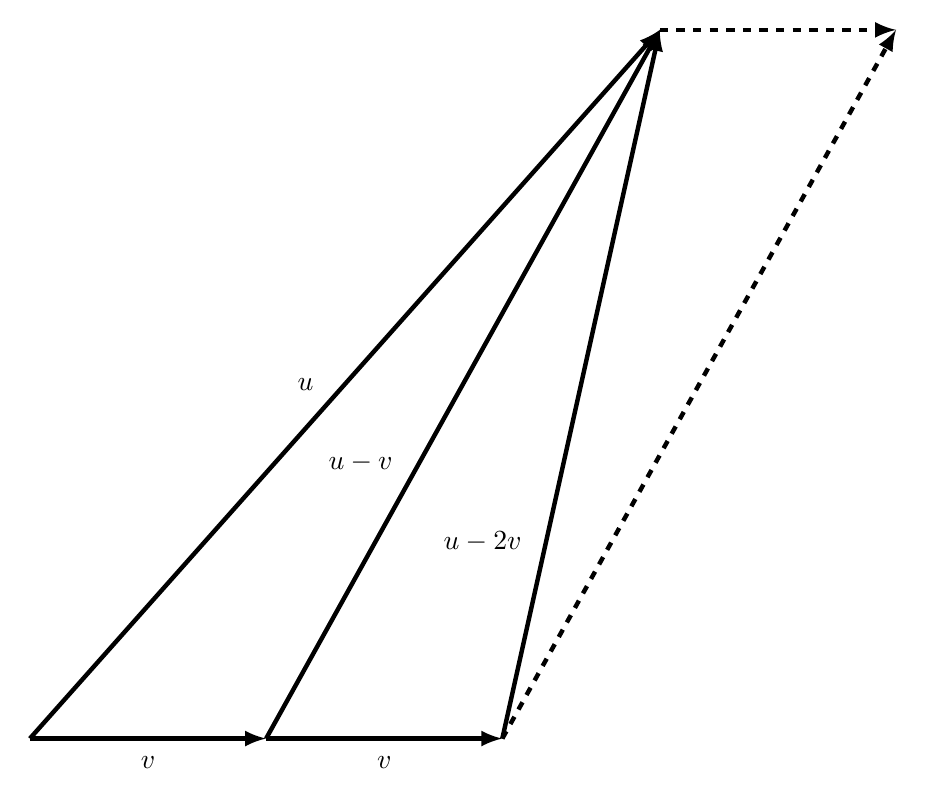
\begin{tikzpicture}
            \draw[-latex, ultra thick] (0, 0) -- (3, 0);
            \draw[-latex, ultra thick] (3, 0) -- (6, 0);
            \draw[-latex, ultra thick] (0, 0) -- (8, 9);
            \draw[-latex, ultra thick] (3, 0) -- (8, 9);
            \draw[-latex, ultra thick] (6, 0) -- (8, 9);
            \draw[-latex, ultra thick, dashed] (8, 9) -- (11, 9);
            \draw[-latex, ultra thick, dashed] (6, 0) -- (11, 9);

            \node at (3.5, 4.5) {\( u \)};
            \node at (1.5, -0.3) {\( v \)};
            \node at (4.5, -0.3) {\( v \)};
            \node at (4.2, 3.5) {\( u - v \)};
            \node at (5.75, 2.5) {\( u - 2v \)};
        \end{tikzpicture}
        \caption{Triangle}
        \label{fig:3}
    \end{figure}
    Set the triangle up as in \Cref{fig:3}, so that
    \[
        \norm{u} = a, \quad \norm{v} = \tfrac{1}{2}c, \quad \norm{u - v} = d, \quand \norm{u - 2v} = b.
    \]
    Consider the parallelogram formed by the vectors \( u - v \) and \( v \). The parallelogram equality states that
    \[
        \norm{u}^2 + \norm{u - 2v}^2 = 2 \norm{v}^2 + 2 \norm{u - v}^2.
    \]
    Substituting the given side lengths, we obtain
    \[
        a^2 + b^2 = \tfrac{1}{2} c^2 + 2 d^2.
    \]
\end{solution}

\noindent \hrulefill

\noindent \hypertarget{ladr}{\textcolor{blue}{[LADR]} Axler, S. (2015) \textit{Linear Algebra Done Right.} 3\ts{rd} edition.}

\end{document}